\chapter{Software Architecture}
\label{ch:Software_Architecture}

While reworking the whole project, a new fundamental software architecture was introduced. This new software stack allows for increased portability, and more important, increased performance. The main principle of this architecture is to separate the reading, preprocessing and storing of the data and the final distribution to the client applications.

\begin{figure}[H]
    \centering
    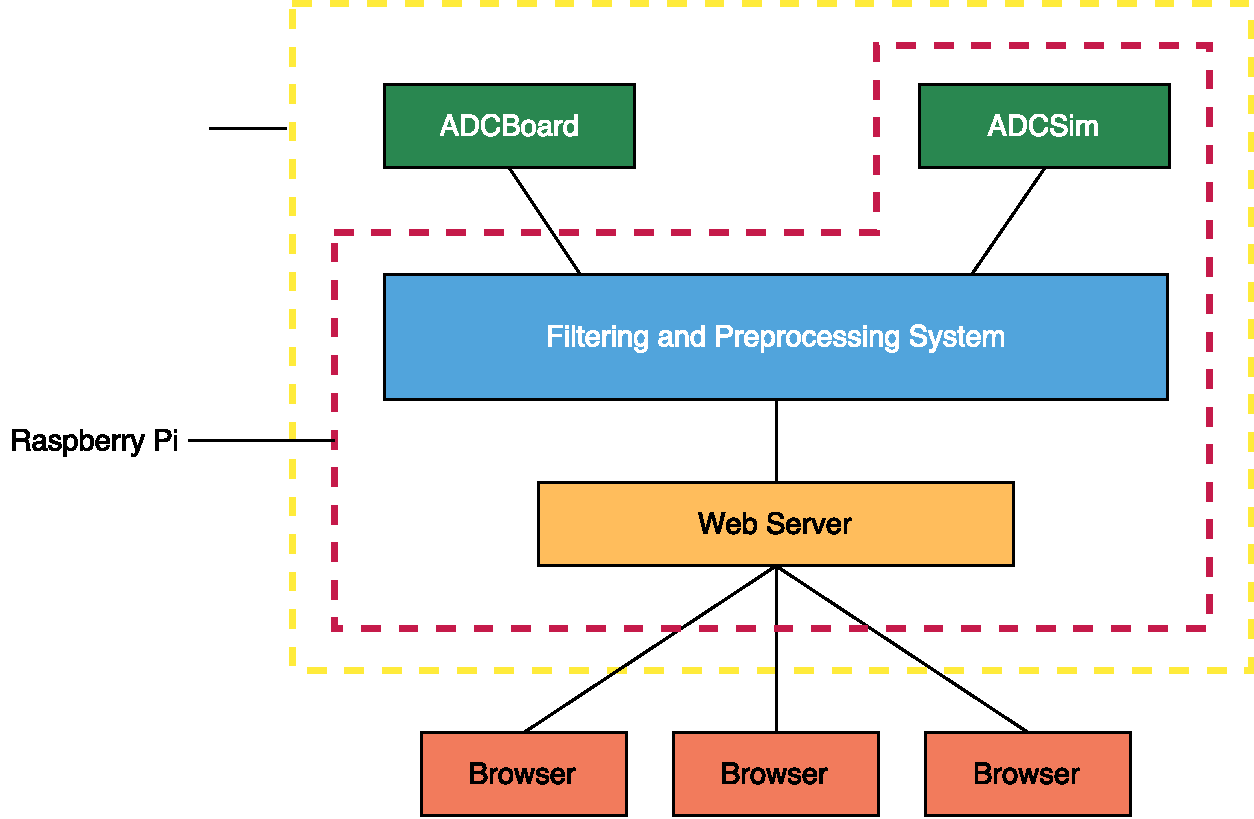
\includegraphics[width=10cm,keepaspectratio]{software_architecture}
    \caption{GRAMOC Software Architecture Diagram}
    \label{fig:software_architecture}
\end{figure}

\section{Readout}

Sensor data is read from a gradient magnetometer. This input is already split into six channels and only has to be converted properly. There are two main inputs that can be used with GRAMOC. The real ADC board and ADCSim, which simulates the board.

\subsection{ADC Board}

This is the component that handles analog to digital conversion, hence ADC board. This circuit board receives analog data from the sensor in six channels. The first three channels being the magnetic field and the last three the gradients.

\subsection{Simulator}

Because the ADC board and a real sensor was not available at all times a simple way of data generation had to be created. Therefore a small application written in C++ was built. This application generates random values and transmits it via UPD just like the real ADC board. Data range and frequency can be adjusted by the user. Another feature that was very important during the development process was the seamless interchangeability with the ADC board.
